% -*- root: ../thesis.tex -*-
%!TEX root = ../thesis.tex
% ******************************* Thesis Chapter 7 ****************************

% ----------------------- paths to graphics ------------------------

% change according to folder and file names
\graphicspath{{7/figures/}}
% ----------------------- contents from here ------------------------



\section{Hawk DLP}

As described above, requirement <insert number> requires Data loss prevention to be added.
According to Hawk terminology, an input abstraction and some vendor-specific inputs need to be added. All of this is realized in the Hawk DLP project. \todo{Include this somehow}

\begin{figure}[!htb]
  \centering

  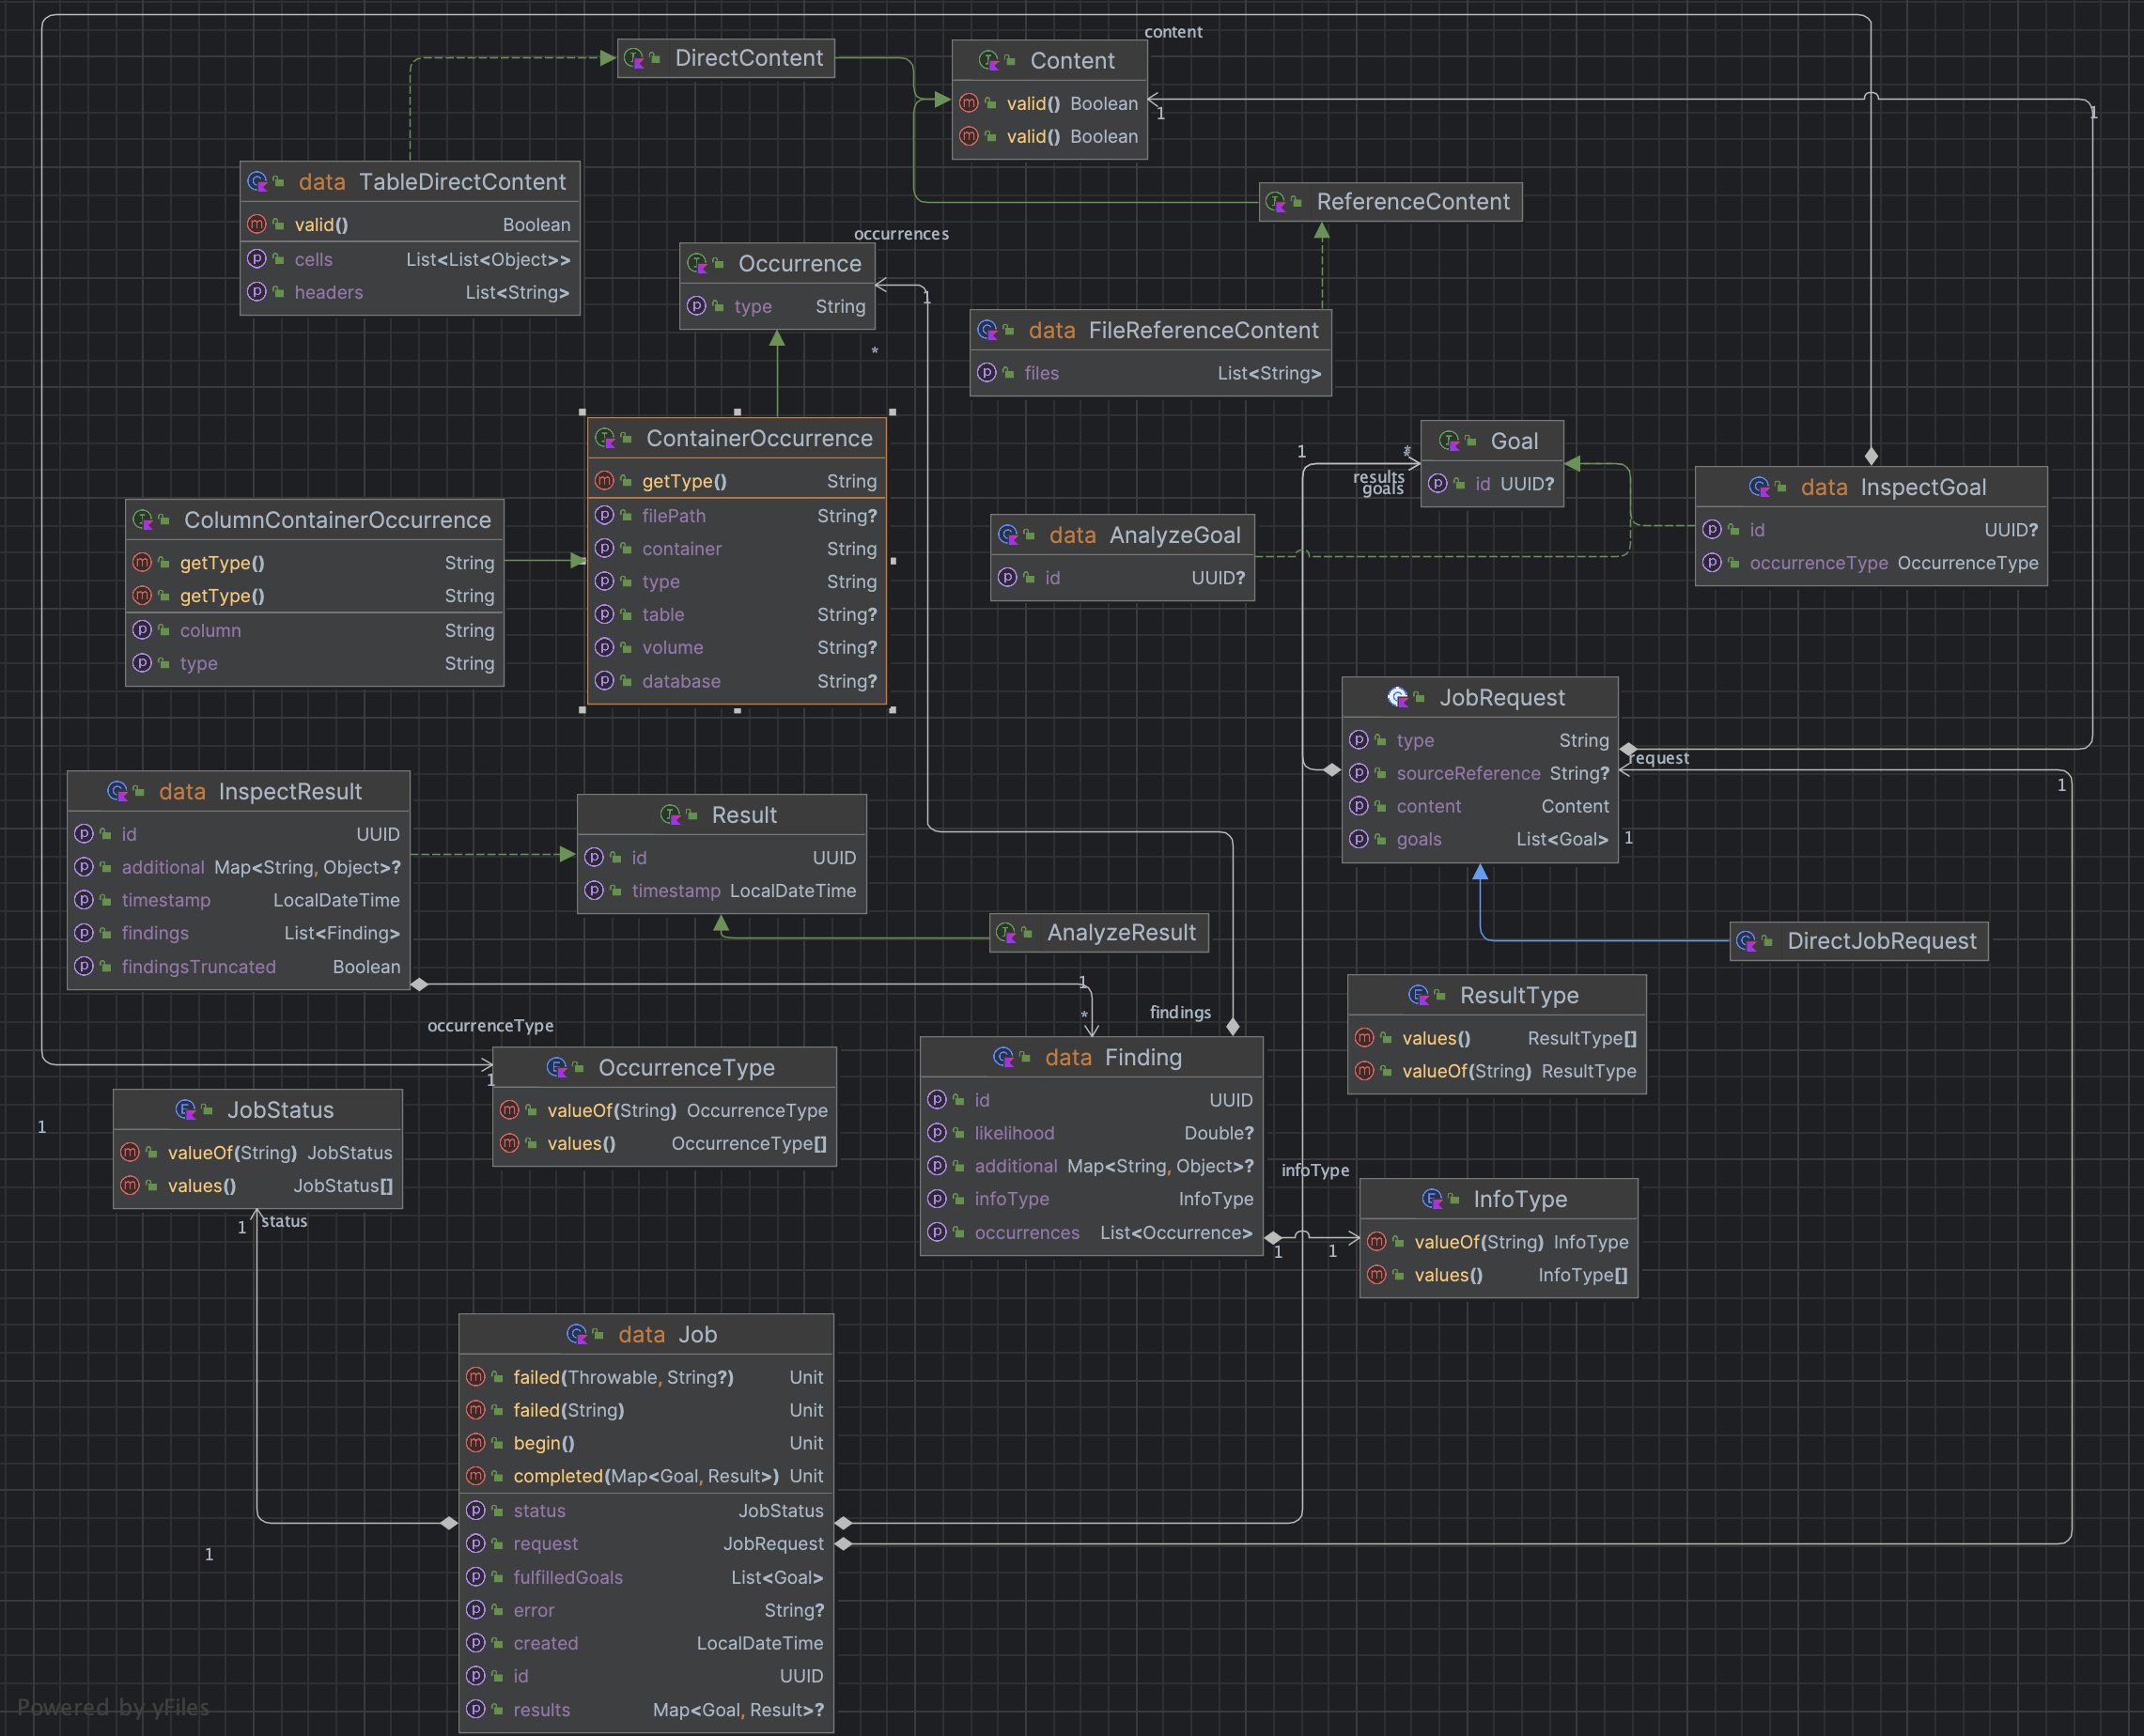
\includegraphics[width=0.95\columnwidth]{hawk-dlp-uml.png}

  \caption[XX]{UML-Diagram of classes in Hawk DLP project}  
  \label{fig:hawk-dlp-uml}
\end{figure}

Both Macie and Google Cloud DLP (CDLP) work by having jobs that get executed asynchronously.
\todo{explain more meta information on what the common module should represent}
\todo{Dont mention jobs cdlp / macie jobs just here yet}

\subsection{Common module}

\todo{Summarize what the common module does}

\subsubsection{Job}
\todo{Introduce why we need jobs}
This means, that a job needs to be created and then continuously queried until the results are present. In both cases, such a job needs to contain a reference to the data/content that should be processed and in some cases additional metadata like a goal. Besides asynchronous Jobs,
CDLP also gives the possibility to embed data directly in the request, that then gets executed synchronously.

To better explain the structure, let's first look at the internal requirements for the project again. The main idea is to build a vendor-independent abstraction above common Data Loss Prevention technologies. The first step to do this is to build a uniform API, which other applications can use, to trigger the vendor-specific jobs and access the results in a common way. This uniform API is also called input abstraction. The second step is to implement the API for different Data Loss Prevention technologies, such as AWS Macie and Google CDLP.

The hawk-dlp-common and hawk-dlp-integration modules represent the input abstraction, with the common module providing the schema and the integration module providing the API.

Now, let's focus on the hawk-dlp-common module again. The first step to implementing these asynchronous jobs is to build a job abstraction for Hawk DLP itself. To define the term clearly, a Job represents a not yet started, a started, or a completed/failed list of tasks. Such a task is a task in the underlying DLP implementation. Note: Don't confuse Hawk DLP jobs with Macie/CDLP jobs.

Jobs can be of different types. In the code, a Job type is represented by the type of the \texttt{JobRequest}, which is also stored as a property in the job class and contains the initial parameters, entered by the user to initiate the Job. The common job type, and for now the only implemented job type is the direct job, represented by the \texttt{DirectJobRequest}. A direct job is as the name suggests a job that gets executed directly and only once after creating the job. The reason for the abstraction is to have the ability to implement other job types in the future. Such other job types could include a scheduled job that gets executed periodically or a trigger-based job for example. The job type name is also present in the \texttt{type} property.

Besides the job type, a job has an id property to uniquely identify the job, a creation date, and a status property. The status property is of type \texttt{JobStatus}, which is an enum and has the following allowed values: 

\textbf{CREATED} is the default status and is present right after the creation of the job.

\textbf{IN\_PROGRESS} is set when the Hawk DLP Integration starts processing the job.

\textbf{COMPLETED} is set when the job is finished successfully. In this case, the (final) result property is present, which will be described later on.

\textbf{FAILED} is set when the processing of the job failed. In this case, a (final) error message in the error property is present.

\textit{final} that the property won't be changed in the status.

\subsubsection{Job Creation}

Now let's take a deeper look at the \texttt{request} property again, which contains the initial job data, provided by the user, that the integration modules use to create the job.
As the \texttt{DirectJobRequest} doesn't add any new properties and the \texttt{JobRequest} class is the superclass of all other job types, we will take a look at the properties of the \texttt{JobRequest} class itself.

The \texttt{content} property can be separated into \texttt{DirectContent} and \texttt{ReferenceContent}, where both classes implement the \texttt{Content} interface. \texttt{DirectContent}, not to be confused with \texttt{DirectJobRequest}, describes the content that is given directly/embedded with the job request (no matter the type of job request). Its size is often restricted due to request/body size limits etc. One concrete example of \texttt{DirectContent} is \texttt{TableDirectContent}, which represents a table that is passed along directly. It is projected by a list of column names and a two-dimensional list of table cells, containing the respective value. \texttt{ReferenceContent} describes the content, which only holds a reference to the content that should be processed. An example here is \texttt{FileReferenceContent}, which contains a reference to a file or a list of files in an e.g. storage bucket.
For now, only the upper mentioned content types exist, with the abstractions in mind to make it possible, to add different types of content in the future. For example, it might be interesting for to add a \texttt{TableReferenceContent} in the future, to represent content in databases.

The \texttt{goals} property contains a list of \texttt{Goal}s. Each goal specifies the anticipated format of the outcome/result of the job being executed. The property allows one job to have multiple results by having multiple goals in the goals list. More on that later.

Finally, the \texttt{sourceReference} property of the \texttt{JobRequest} class contains a user-set string that marks the origin of the data being processed. In case of direct content, for example, it might not be clear from outside, where the content that is processed came from. But also for reference content, it's sometimes helpful, e.g. when aggregated data gets processed. The property is important for the Hawk Service in the next section.

\subsubsection{Job Execution}

With the \texttt{JobRequest} and the process of representing the job creation in the code explained, the next step is to explain the job execution and the way outcomes/results are represented. In the code, the instance of the job object gets forwarded to the integration. The integration then mutates the job instance and updates the \texttt{status}, \texttt{results}, and \texttt{error} properties. As explained above, right when the integration starts processing the job, the \texttt{status} property is set to \texttt{CREATED}.

To understand how the results are represented in the code, it's important to understand how results of the DLP tools themselves look like. Many DLP technologies share a similar set of features, where each feature works by providing input data and extracting the result after execution. With one of those being the so-called inspection feature. As explained earlier \todo{Explain this in prev part}, it works by inspecting data like for example tables and returns where which type of data was identified, e.g. column x in table y is of data type email. Another feature supported by some DLP tools is called analyzation, which extracts certain privacy metrics.

Since Hawk DLP builds above other DLP tools, those features must be somehow represented. For this reason, we have the \texttt{Goal} interface and \texttt{Result} interface, with subtypes of those representing a specific DLP feature. The goal represents a feature-specific list of parameters, on how to perform the feature and format the result afterward. It is provided in the job creation process, alongside the \texttt{Content} that should be processed. When processing is done, depending on the list of goals provided and whether the DLP implementation supports it, each goal gets a result associated with it.

As mentioned earlier, the main feature that we want to support is the inspection feature \todo{name inspection feature like in earlier sections}. It is implemented by the \texttt{InspectGoal} and \texttt{InspectResult} classes. The feature works by inspecting the content provided and returning a list of findings, where what type of data can be found. Such a type of data could be \texttt{EMAIL}, which is represented in the \texttt{InfoType} enum. Besides the info type, some DLP implementations also give a probability, to which this info type is accurate. Hawk DLP represents this by a double between 0 and 1, where 1 is very likely. The location, where the info type was found in the supplied \texttt{Content}, is represented by sub-types of the \texttt{Occurrence} interface. 

\todo{Better introduction} There is therefore a certain relation between the \texttt{Content} sub-type supplied and the \texttt{Occurrence} sub-type returned. For table-based content, there is the \texttt{ColumnContainerOccurrence}. For document-based content, another sub-type could be created in the future. The \texttt{ColumnContainerOccurrence} is based on the \texttt{ContainerOccurrence}, which contains a locator for the file, database table etc. of the finding. To create a vendor-independent interface, this interface specifies some other properties. 
For file occurrences, the \texttt{volume} and \texttt{filePath} properties are presented. The first describe the location, where the file (system) of the file is located at. E.g. the name of a storage bucket. The latter describes the path of the file in the respective volume.
For (managed) database occurrences, \texttt{database} and \texttt{table} properties are present. The \texttt{database} property describe all the prefixes of the table itself. This could be a project name, depending on the database a database name and / or a schema etc. The \texttt{table} property simply describes the name of the table.
As earlier mentioned, table content has a specific type of occurrence - \texttt{ColumnContainerOccurence}. They inherit all properties from the \texttt{ContainerOccurence} and a \texttt{column} property for the column in the managed database / (CSV) file etc.
In the future, it is possible also to add a \texttt{CellContainerOccurence}, which could contain a row identifier besides the column name and allow for a cell specific inspection of the data.

To reduce redundant data, occurrences with the same info type (and if present likelihood) get aggregated in the same finding. Meaning a finding has a list of occurrences. The \texttt{InspectResult} simply contains a list of \texttt{Finding}s and a boolean, whether any findings were excluded or not (some might be excluded because of size limits etc.). Depending on the implementation some additional properties might exist in the \texttt{InspectResult}, \texttt{Finding} and / or \texttt{Occurrence} classes. To transform the result from the DLP implementation it is required to specify the \texttt{OccurrenceType} in the \texttt{InspectGoal}.

A second feature, which is not yet implemented, but support by some DLP technologies is the analyzation features. It calculates certain privacy metrics from the data supplied. \todo{Describe this better}. For future implementation the \texttt{AnalyzeGoal} and \texttt{AnalyzeResult} classes were already added.

To enabled multiple types of results by one execution, the \texttt{JobRequest} gives the possibility to specify multiple \texttt{Goal}s in the request. This results in one \texttt{Result} being created for each \texttt{Goal}.

Now, back to the job execution process. Job Status is changed to \texttt{IN\_PROGRESS}, when the request was passed to the integration. The integration then extracts the request and passes the data to the DLP implementation. When the DLP implementation responds with a result, the integration parses it according to the \texttt{Goal}s provided and fills the \texttt{results} map in the \texttt{Job} class. In this case, the \texttt{JobStatus} gets updated to \texttt{COMPLETED}. In case of an error, the \texttt{FAILED} \texttt{JobStatus} is set and there error messages is saved in the \texttt{error} property.

\todo{add example with a table}

\subsection{Integration Module}

The integration module simply adds a base module for all integrations. Since integratration modules expose a uniform REST API and use the Spring Boot Framework, it abstracts the presentation layer (according to DDD) \todo{Cite DDD} and provides some a interface for extension. The integration module depends on the common module and uses its types for abstraction. 

\paragraph{REST API}
Different endpoints are defined in the \texttt{JobController}. All of them provide CRUD-based operations for the Job entity or any of its sub-entities.
\todo{Add OpenAPI}

The first category of endpoints is used to create jobs. As described in the common module, different Job types exist. In the API this is represented by one endpoint per Job type. Currently, only one Job type exists - the direct job type. This means that the only endpoint is the \texttt{direct job create} endpoint. It is accessible under \texttt{POST /api/v1/jobs/direct}. As a request body, a \texttt{DirectJobRequest} must be provided as JSON. When the input is valid, a \texttt{Job} instance will be returned as a result.

The second endpoint is to list all cached \texttt{Job}s. Each instance of the Hawk DLP integration stores a list of that are/were processed by it. Currently, this list is volatile. In the future, this could be easily implemented with persistence, to enable browsing older jobs and achieve horizontal scalability of Hawk DLP integration instances. The endpoint is accessible under \texttt{GET /api/v1/jobs}

To inspect single job instances, the \texttt{GET /api/v1/jobs/\{id\}} endpoint can be used. The path variable \texttt{id} represents the \texttt{id} property of the \texttt{Job} class returned by a job create endpoint. This endpoint should be used to access completed jobs and/or monitor jobs in progress.

Since some properties are suppressed in the JSON view of the \texttt{Job} due to their size, some get endpoint for the sub-entities of the \texttt{Job} class exists.
Namely, the \texttt{request} and the \texttt{results} properties are suppressed. The first can be accessed by \texttt{/request} as a suffix - \texttt{GET /api/v1/jobs/\{id\}/request}. The latter represents a list of results. Therefore, the \texttt{GET /api/v1/jobs/\{id\}/results} endpoint only returns a list of result ids available to this job. By specifying the result id in \texttt{GET /api/v1/jobs/\{id\}/results/\{resultId\}}, the individual \texttt{Result} can be accessed.

\subsubsection{Job API}

To forward requests of the REST API to the concrete integration implementation, an abstraction is provided. The \texttt{JobService} class holds a \texttt{Map} of stored jobs by this Hawk DLP integration instance. When an endpoint is called, the response is served by accessing or modifying this \texttt{Map}. Besides adding a Map-Entry when creating a job via. any of the job create endpoints, a Spring event is published in the Spring \texttt{EventBus}. Integration implementations can listen to the \texttt{JobCreatedEvent} being published in the Event bus, holding the \texttt{Job} instance and start processing the request. The \texttt{Job} instance will be mutated by the Integration implementation, which leads to the endpoints immediately serving the new content.

\subsection{Google Cloud DLP 2 module}
The Google Cloud DLP is a Data loss prevention tool developed by Google and offered in the Google Cloud Platform. This module represents 


\subsection{AWS Macie 2 module}



\section{Hawk API \& Hawk Service}

\todo{Figure: File tree of the hawk service to show package by feature}
Similar to the previous Hawk, the Hawk Service is a core component of the Hawk Framework. It serves the Hawk API, which can be used to access data from the technologies behind Hawk in a uniform way. One of the main contributions to the Hawk Service is the encapsulation of inputs and outputs. The project still follows a strict package-by-feature layout, but with all of the old classes grouped into a traffic-analysis package. The release module, is encapsulated into a \texttt{module/release} package. Along with it some module classes itself were abstracted, to be reused in other modules.

\subsection{Hawk DLP integration}
In order to enable the Hawk API to return information extracted via DLP tools, Hawk DLP inputs have to communicate with the Hawk Service. This communication works by letting the Hawk API expose a Hawk-DLP-Job-Update endpoint. This endpoint receives Hawk DLP Jobs parses them with available internal modules and then persists those changes into a database. Using the data persisted in this database, the Hawk API can access all saved jobs.

The transmission of the DLP-Jobs can be optionally enabled in the Hawk DLP input. By default its disabled, to have the ability to run Hawk DLP autonomously. 
In detail, this realized, by having the integration module of the Hawk DLP project providing an interceptor, that can be enabled to send all Job updates to the Hawk Service. In this case, the REST-API of the Hawk DLP input still works normally. The reason for the push-based approach in terms of pushing Job-update to the Hawk Service, is to enable running multiple different Hawk DLP inputs, without having to register each one at the Hawk Service. Alternatively, a pull-based approach would be possibile, which would bring the challenge coordinating Job-Update-Reqeuests when having multiple Hawk Service instances running. By using the push-based approach, the only stateful component is the database, which makes the whole application horizontal scalable and cloud-native.

\subsection{Hawk Cluster detection module}
Another new contribution of the new Hawk Service is the Cluster detection module.
As mentioned above, many companies today are using microservices. The idea of a Microservice is to handle a small part of a bigger application. A core requirement of the Microservice architecture is encapsulation, which results in many Microservices having their own (private) components, such as databases etc. Since there is no 100-percent accurate way of identifying to which Microservice a database for example belongs to, the Hawk Cluster detection module introduces a \texttt{hawk.io/app-name} label. This label is only available in Kubernetes-based environments.

The cluster detection module, works by resolving the above mentioned label from the component present in the context. In case of a DLP Job, such a context could be the \texttt{JobRequest.sourceReference} property. In case of traffic analysis, which is already present in the old Hawk Framework, it could \texttt{Usage.endpointHost}. The cluster detection module then uses the Kubernetes API to identify \texttt{Pod}s, \texttt{Service}s, \texttt{EndpointSlice}s or the current \texttt{Namespace} from the context in order to resolve the label value. The cluster detection module then tags the DLP Jobs / Traffic-Analysis Usages with this app-name value. Based on those tags queries can be made, as explained in the next section. \todo{mention that service meshes like istio or the osm standard are not yet supported; mention the approach is watcher based to save requests to the kubernetes api}

\subsection{Hawk API}
As covered in previous sections, the Hawk API is a collection of new endpoints available to the Hawk Service.
Those endpoints follow the REST paradigm and are primarily grouped by their respective feature (dlp, traffic analysis, app etc.) and secondarily by their layer (input, output). The Hawk API can therefore separated into the following categories / features:

\subsubsection{Traffic Analysis [Input,Output?]}

\subsubsection{Data Loss Prevention [Input,Output]}
- similar to (volatile) REST API on Hawk DLP input itself, but with filter capability and persistence (and tagged data from modules). 

\subsubsection{Release [Output]}
- find all data gathered in a specific release (see release module)

\subsubsection{Application [Output]}
- find all data (traffic analysis and data loss prevention) for a specific app label name (see cluster detection module).
\todo{first real (strong) synergy effects!}

\section{Outputs}
\subsection{Data Protection Impact Assessment Generator}
\section{Deployment}


\todo{add glossary for abkürzungen}
\todo{add examples for each section}

% ---------------------------------------------------------------------------
% ----------------------- end of thesis sub-document ------------------------
% ---------------------------------------------------------------------------